% Turn on subsection numbering.
\setsecnumdepth{subsection}

% Default styles.
\aliaspagestyle{title}{empty}
\aliaspagestyle{chapter}{empty}
\aliaspagestyle{part}{empty}

% Use normal font for URLs.
\renewcommand\UrlFont{\normalfont}

% -----------------------------------------------
% Chapter thumb style
% -----------------------------------------------

% Add a layer so that the chapterthumb.sty package can insert the thumb index.
% Also set the font style to bold for better readability.

\pagestyle{scrheadings}
\AddLayersToPageStyle{scrheadings}{chapterthumb}
\addtokomafont{chapterthumb}{\bfseries}

% -----------------------------------------------
% Header style
% -----------------------------------------------

% By default the headers are uppercase, headings on the left page show the
% chapter number and name, headings on the right page show the closest section
% name. Because sections in a thesis usually don't last for many pages these
% were removed. The remaining headings are set to lowercase with appropriate
% uppercasing of first letters.

\pagestyle{headings}
\nouppercaseheads
% Remove header for odd numbered pages.
\renewcommand\sectionmark[1]{\markright{}}

% -----------------------------------------------
% Abstract style
% -----------------------------------------------

% Define abstract boxes. Defines a new environment 'boxabstract' that wraps the
% abstract text into a gray box with a dark abstract label on top.

\definecolor{lightgray}{RGB}{230,230,230}
\definecolor{darkgray}{RGB}{0,0,0}

\usetikzlibrary{shapes}

\newcommand{\boxabstract}[2][]{
  \begin{center}
    \begin{tikzpicture}
      \node(box)[fill = lightgray, rectangle, inner sep = 10pt, rounded corners = 1]{%
        \begin{minipage}{12.05cm}
          \setlength{\parindent}{1em}
          {\vspace*{3pt} #2}
        \end{minipage}%
      };
      \node[fill = darkgray, text = white, right = 10pt, inner sep = 5.5pt] at (box.north west) {\textsf{\textbf{Abstract}}};
    \end{tikzpicture}
  \end{center}
}

% -----------------------------------------------
% Chapter style
% -----------------------------------------------

% For a somewhat short introduction and a couple of examples check:
% http://ctan.cs.uu.nl/info/latex-samples/MemoirChapStyles/MemoirChapStyles.pdf
% https://texblog.org/2012/07/03/fancy-latex-chapter-styles/
% The example below is a custom styling that uses various fonts and font sizes.

\makeatletter

\makechapterstyle{myveelo}{
  \setlength{\afterchapskip}{40pt}
  \renewcommand*{\chapterheadstart}{\vspace*{40pt}}
  \renewcommand*{\afterchapternum}{\par\nobreak\vskip 25pt}
  \renewcommand*{\chapnamefont}{\normalfont\itshape\Large}
  \renewcommand*{\chapnumfont}{\normalfont\itshape\HUGE}
  \renewcommand*{\chaptitlefont}{\normalfont\HUGE\bfseries\flushright}
  \renewcommand*{\printchaptername}{\flushright\chapnamefont\MakeUppercase{\@chapapp\hspace*{6pt}}}
  \renewcommand*{\chapternamenum}{}
  \setlength{\beforechapskip}{18mm}
  \setlength{\midchapskip}{\paperwidth}
  \addtolength{\midchapskip}{-\textwidth}
  \addtolength{\midchapskip}{-\spinemargin}
  \addtolength{\midchapskip}{-11.5em}
  \renewcommand*{\printchapternum}{%
    \enspace\resizebox{!}{10mm}{\chapnumfont\thechapter}%
    \rlap{\hspace{1cm}\rule{\midchapskip}{\beforechapskip}}%
  }%
  \makeoddfoot{plain}{}{}{\thepage}%
}

\chapterstyle{myveelo}
\makeatother

% -----------------------------------------------
% Part style
% -----------------------------------------------

\renewcommand*{\partnamefont}{\normalfont\itshape\LARGE}
\renewcommand*{\partnumfont}{\normalfont\itshape\HUGE}
\renewcommand*{\parttitlefont}{\normalfont\HUGE\bfseries}
% Print part #num, e.g. 'part 1'.
\renewcommand*{\printpartname}{\partnamefont\MakeUppercase{\partname}}
% Print nothing except for the part heading.
% \renewcommand*{\printpartname}{}
% \renewcommand*{\printpartnum}{}

% -----------------------------------------------
% Chapter and part backgrounds
% -----------------------------------------------

% Defines two switches, one for chapter backgrounds and one for part
% backgrounds. Backgrounds can fill a whole page, the included examples show how
% to restrict to smaller areas. With the examples below chapter backgrounds fill
% two pages, the first will be on the left and the second will be backing the
% chapter layout elements (header, footer, etc.). The part background has a
% background on the left and the part header without a background on the right.

% Chapter background:
% \cleartoverso
% \backgroundtrue
% \cleartorecto
% \chapter{Description of Chapter}
% <chapter layout elements go here>
% \clearpage
% \backgroundfalse

% Part background:
% \cleartoverso
% \partbackgroundtrue
% \cleartorecto
% \partbackgroundfalse

\newif\ifbackground
% Chapter page backgrounds
\AddToShipoutPictureBG{\ifthenelse{ \isodd{\value{page}} \AND \boolean{background} }{\AtStockLowerLeft{
\includegraphics[width=21cm]{chapter-backgrounds/background-chapter-right}}}{}}
% accross chapter page background
\AddToShipoutPictureBG{\ifthenelse{ \NOT\isodd{\value{page}} \AND \boolean{background} }{\AtStockLowerLeft{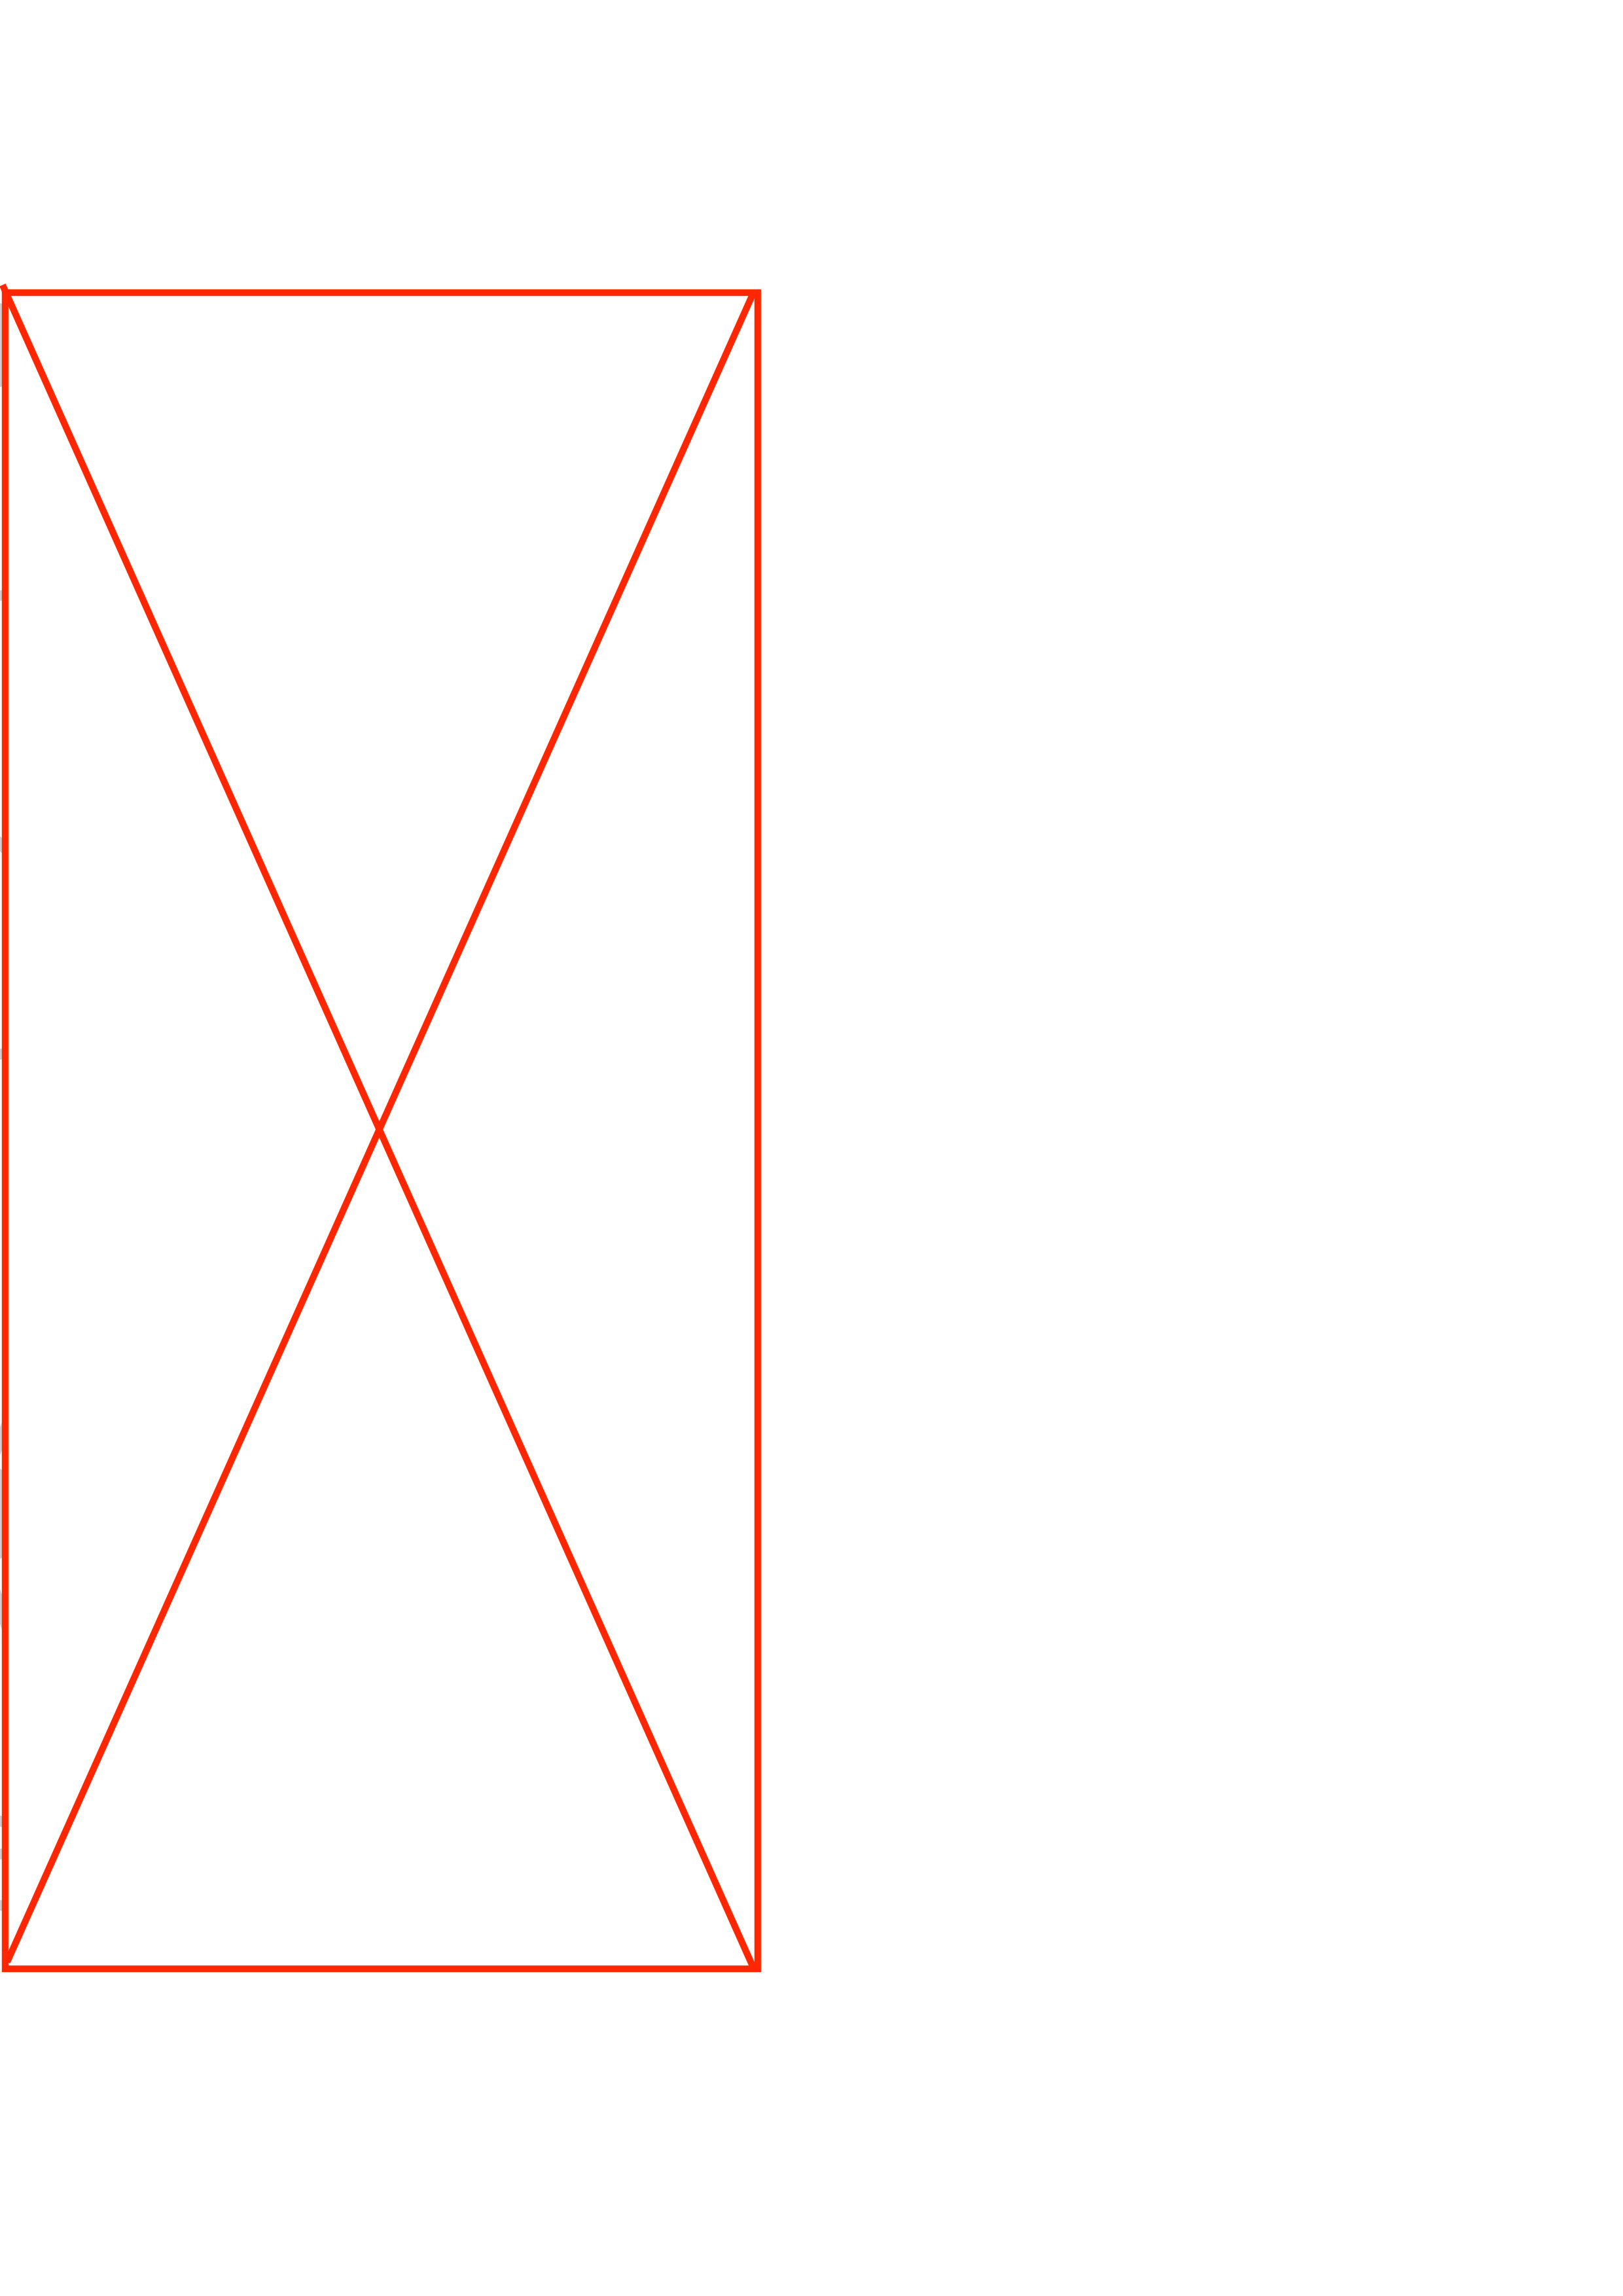
\includegraphics[width=21cm]{chapter-backgrounds/background-chapter-left}}}{}}
% accross part page background
\newif\ifpartbackground
\AddToShipoutPictureBG{\ifthenelse{ \NOT\isodd{\value{page}} \AND \boolean{partbackground} }{\AtStockLowerLeft{
\includegraphics[width=21cm]{chapter-backgrounds/background-part}}}{}}